\documentclass[11pt, letterpaper]{report}

%paquetes
\usepackage{tikz}
\usepackage{xcolor}
\usepackage{graphicx}
\usepackage{amsmath}
\usepackage{amssymb}
\usepackage[spanish, activeacute]{babel}
\usepackage{colortbl}
\usepackage{float}
\usepackage[utf8]{inputenc}
\usepackage[right = 2.5 cm, left = 2.5 cm, top = 2 cm , bottom = 2 cm]{geometry}
\usepackage{enumitem} %sirve para cambiar el tipo de enumeracion si redefinir comandos ejem: \arabic* \alph*

%configuraciones
\renewcommand{\labelenumi}{$\bullet$} 
\newenvironment{enumTab}{\begin{enumerate}[label=]\item \begin{enumerate}[label=$\bullet$]}{\end{enumerate}\end{enumerate}} %comando para realizar enumeraciones con cierto margen
\newenvironment{block}[1]{\hspace{-0.8 cm}\textbf{\Large #1}}{\vspace{3 mm}} %ambiente importante que define una parte del reporte.
\newenvironment{question}[2]{\hspace{-0.8 cm}\textbf{#1) #2\\\\}}{\vspace{3 mm}} % define una pregunta, recibe como primer parametro al número y siguiente es la pregunta
\newcommand{\bib}[2]{ \textbf{\large #1:} \small #2\\} %forma sencilla de crear una referencia, como primer parametro recibe el titulo y el segundo el lugar a consultar
\newcommand{\note}[1]{\small \textbf{Nota:} #1} %comando que inserta una nota al texto
\spanishdecimal{.}
%comandos personales
%este commando sirve para crear bolas con enumeración
\newcommand*{\enumBall}[1]
		{
		\footnotesize\protect\tikz[baseline=-3pt]
		\protect\node[scale=.7, circle, ball color = white]{\color{black}\Large\bf #1};
		}

\begin{document} 
	%%%% BLOQUE DE DATOS %%%

\newcommand{\Title}{
	Guía de Usuario para Report
} %Titulo del reporte

\newcommand{\LogoUniversity}{img/logo.jpg} %logo de la universidad
\newcommand{\NameUniversity}{Universidad Galileo} %Nombre de la universidad
\newcommand{\Date}{
	Guatemala, 6 de marzo de 2020
} %Fecha de entrega
\newcommand{\Faculty}{Facultad FISICC} %Nombre de la facultad
\newcommand{\Course}{
	Curso: *******
} %Nombre del curso
\newcommand{\ID}{
	Carnet: **** ****
}
\newcommand{\Student}{
	Alumno: Josué Benyamin Isaí Galeano Morales
} %Nombre del estudiante
\newcommand{\Section}{
	Secci\'on: *
} %Sección del estudiante
\newcommand{\Schedule}{
	Horario de laboratorio: 18:00 a 19:00
} %Horario
\newcommand{\Assistant}{
	Auxiliar: *******
} %Persona encargada
\newcommand{\Day}{
	Día de laboratorio: viernes
} %Dia en que recibe
%% FIN BLOQUE DE DATOS%%


%% NO ES NECESARIO MODIFICAR ESTA PARTE %%
\def\arraystretch{1.2}
\textbf{
	\small
	\hspace{-1 cm}
	\begin{minipage}{0.15\textwidth}
		%%%%%%%%%%%%%%%%% LOGO %%%%%%%%%%%%%%%%%%%%%%%%%%%%%%%
		\includegraphics[scale=0.5]{\LogoUniversity}
	\end{minipage}
	\begin{minipage}{0.7\textwidth}
		\resizebox{1.25\textwidth}{!}{
			\begin{tabular}{ll}
				\hline 
				%%%%% PARTE SUPERIOR DE LA TABLA DE DATOS %%%%%%%%%%%%%%%%%%%%%%%
				\NameUniversity & \Date \\
				\hline
				\rowcolor{lightgray}
				\Faculty & \Student\\
				\hline 
				\Course & \ID\\
				\hline\rowcolor{lightgray}
				\Section & \Schedule\\
				\hline 
				\Assistant & \Day\\
				\hline
			\end{tabular}
		}
	\end{minipage}
}

\vspace{0.5cm}
\begin{tikzpicture}
\hspace{-1 cm}
\draw (0.1,0.1) rectangle (1.043\textwidth,0.9);
\draw[line width=0.7mm] (0,0) rectangle (1.05\textwidth,1);
\node[font=\Large] at (0.525\textwidth, 0.45) {\textbf{\Title}};
\end{tikzpicture}		

\def\arraystretch{1}

\vspace*{0.5 cm}
 %incluimos la parte del header en el documento, note que header es como escribir dentro de un ambiente document por lo tanto no debe llevar definición de clase ni definiciones que se hagan exclusivamente en el preambulo.
	
	 \begin{block}{Objetivos:}
	 \begin{enumTab}
			
	\item Que el estudiante se familiarice con los divisores de corriente y voltaje para formar un concepto sólido de la proporción entre resistencia , voltajes y corrientes en un circuito.
	\end{enumTab}
	 \end{block}
		
	\begin{block}{Resumen:}
		
		En la pr'actica calculamos de manera te'orica los voltajes, corrientes, resistencias equivalentes, etc. mediante las herramientas conocidas como \textbf{\emph{Divisores}} las cuales ayudan a hacer un an'alisis m'as f'acil en la mayoria de casos. 
	\end{block}
		
	\begin{block}{Teor'ia:}
	
	  \textbf{Los circuitos Serie} son una configuraci'on especial de componentes en un circuito, la caracter'istica de estos circuitos es que la corriente que fluye por todos sus miembros es la misma, por lo mismo la resistencia equivalente de resistores en serie es la suma de sus valores debido a que todos ellos se oponen a la misma corriente, a partir de la ley de Voltajes de \emph{Kirchhoff} se puede deducir la herramienta \textbf{\emph{divisor de voltaje}}:
	  
	  \begin{figure}[H] %H obliga que la figura est'e exactamente en este lugar.
	  \[V_i = V_f \biggl( \frac{R_i}{R_{\tiny EQ}} \biggr)\]
	  \caption{\textbf{\emph{ecuaci'on de divisior de voltaje}}}
	  \end{figure}
	  
	\begin{figure}[H]
	\hfill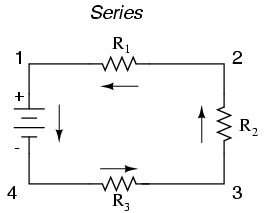
\includegraphics[scale=0.5]{img/serie.png}\hspace*{\fill}
	\caption{\textbf{\emph{Circuito Serie}}}
	\end{figure}
	
	\textbf{Los circuitos en paralelo} tienen como caracter'istica especial que comparte un mismo voltaje, debido a que tienen dos nodos en com'un la tensi'on debe ser la misma para todos, gracias a la ley de corrientes de \emph{Kirchhoff} se puede deducir la segunda herramienta conocida como \textbf{\emph{divisor de Corriente}}:

		\begin{figure}[H]
		\[I_i = I_f \biggl( \frac{R_{\tiny EQ}}{R_i} \biggr)\]
		\caption{\textbf{\emph{ecuaci'on de divisor de Corriente}}}
		\end{figure}
	
		 \begin{figure}[H]
		 \hfill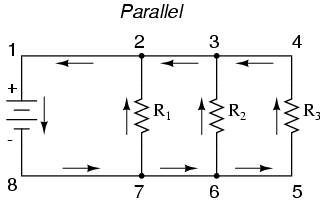
\includegraphics[scale=.5]{img/paralelo.png}\hspace*{\fill}
		 \caption{\textbf{\emph{Circuito Paralelo}}}
		 \end{figure}
	\end{block}
		
	%datos practicos
	\begin{block}{Datos Pr'acticos:}
	
	En la siguiente imagen se podr'a ver la construcci'on del circuito proveido en la pr'actica, tambi'en se muestra la Resistencia ``Pr'actica" que cae sobre el circuito.
	
	\begin{figure}[H]
	\hfill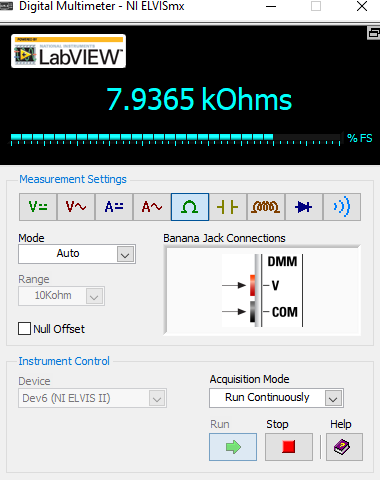
\includegraphics[width=.32\textwidth]{img/image.png}\hspace*{\fill}
	\caption{\textbf{\emph{Resistencia equivalente del 'ultimo circuito}}}
	\end{figure}
	
	\begin{figure}[H]
	\hfill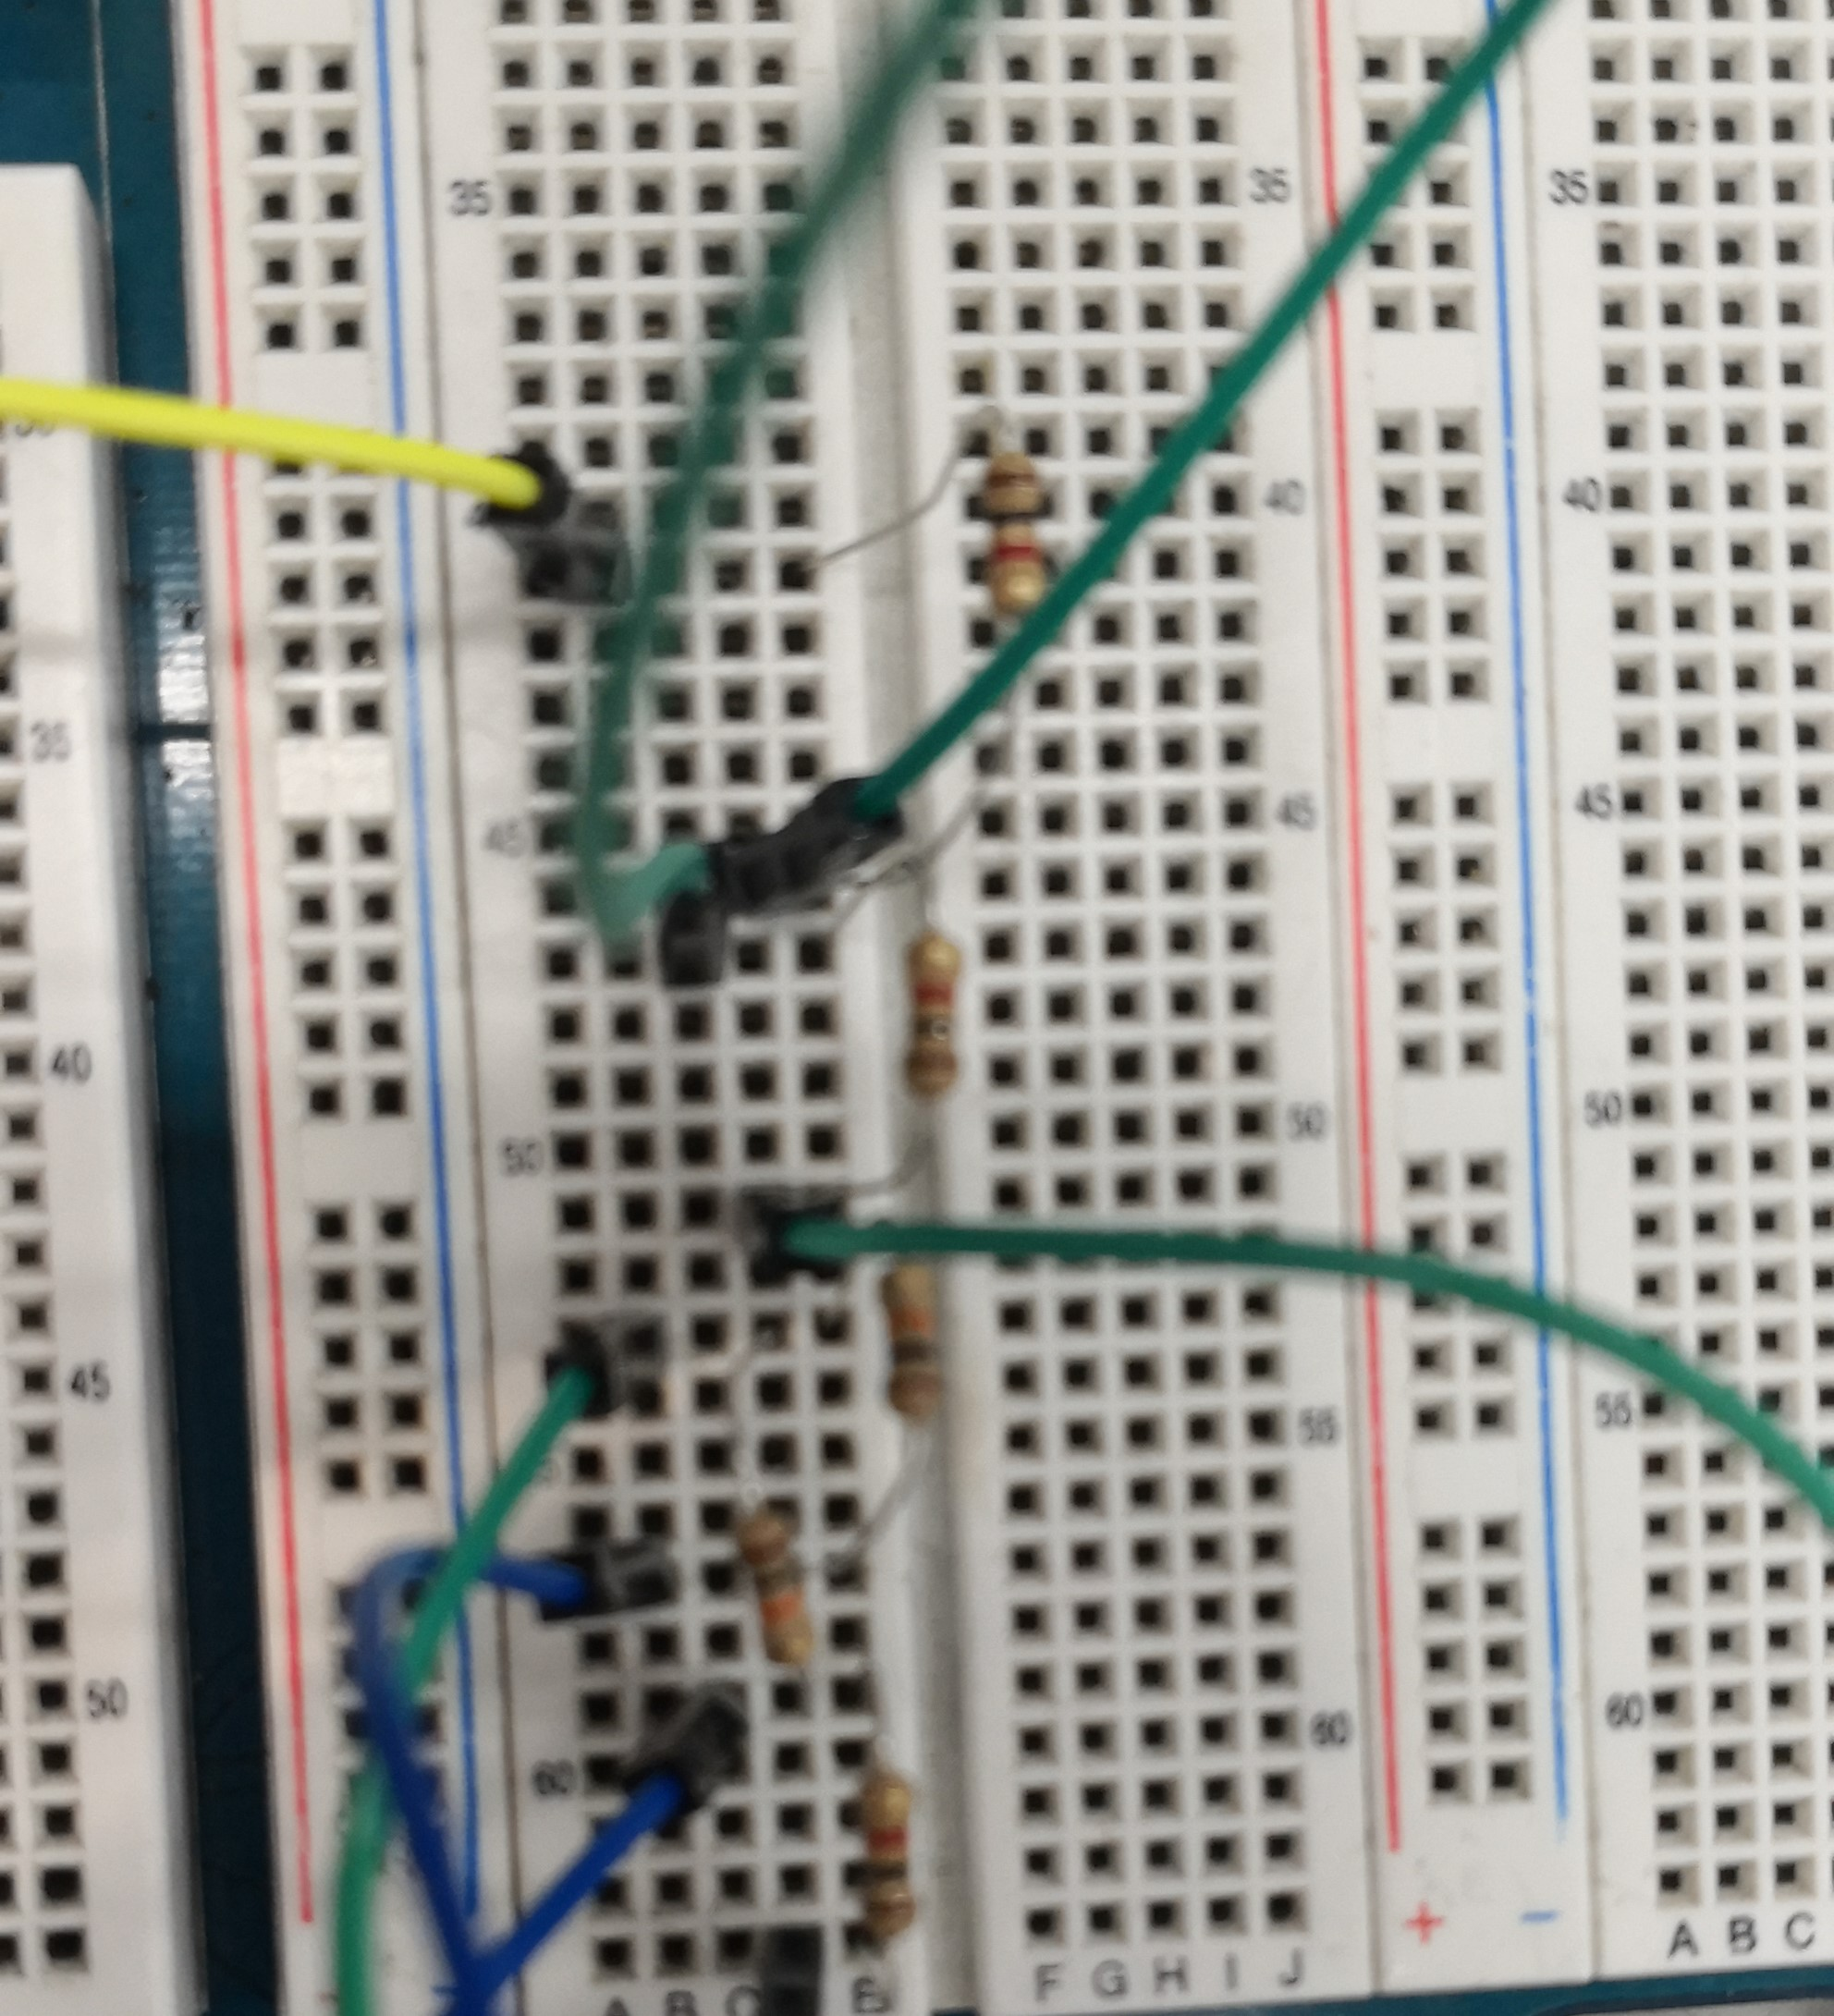
\includegraphics[width=.32\textwidth]{img/circ.jpg} \hspace*{\fill}
	\caption{\textbf{\emph{circuito físico (el 'ultimo)}}}
	\end{figure}
	
	\note{debido a que las puntas que usaba en la pr'actica no estaban buenas y no me percat'e a tiempo no me dio tiempo de realizar m'as cosas.}
	
	\end{block}
	
	
	\begin{block}{C'alculos Te'oricos:\\}
	
	
	{\large \bfseries{Incisos Laboratorio \#4\\}}
	
	\begin{question}{4}{an'alisis del circuito 1}
	\(R_{EQ}=1k\Omega+4.7k\Omega=5.7k\Omega\); \(I_f=\frac{V_f}{R_{EQ}}=\frac{5V}{5.7k\Omega}=877\mu A\)\\
	\(V_x=R_xI_f=(1k\Omega)(877\mu A)=877mV\); \(V_y=R_yI_f=(4.7k\Omega)(877\mu A)=4.12V\)
	
	\vspace{.5 cm}
	\begin{tabular}{cccc}
	\hline
	Voltaje & valor te'orico. & valor pr'actico. & Error (\%)\\
	\hline\hline
	\(V_x\) & 877mV & --- & ---\\
	\hline
	\(V_y\) & 4.12V & --- & ---\\
	\hline
	\end{tabular}

	\end{question}
	
	\begin{question}{6}{mismos calculos del inciso 4, pero con \(R_x = 4.7k\Omega\)}
	
	\(R_{EQ}=4.7k\Omega+4.7k\Omega=9.4k\Omega\); \(I_f=\frac{V_f}{R_{EQ}}=\frac{5V}{9.4k\Omega}=532\mu A\)\\
	\(V_x=R_xI_f=(4.7k\Omega)(532\mu A)=2.5V\); \(V_y=R_yI_f=(4.7k\Omega)(532\mu A)=2.5V\)
	
	\vspace{.5 cm}
	\begin{tabular}{cccc}
	\hline
	Voltaje & valor te'orico. & valor pr'actico. & Error (\%)\\
	\hline\hline
	\(V_x\) & 2.5V & --- & ---\\
	\hline
	\(V_y\) & 2.5V & --- & ---\\
	\hline
	\end{tabular}
	\end{question}
	
	\vspace{3 mm}
	\begin{question}{7}{Calcular}
	La resistencia total del circuito se puede escribir de la siguiente forma: \(R_{EQ}=3k\Omega+R_?\) siendo \(R_?=R_1||R_2\), calculemos entonces a \(R_?\)\\
	\[3V=12V\bigl( \frac{2k\Omega}{3k\Omega+R_?} \bigr)\] \[3V(3K\Omega + R_?)=24VK\Omega\] \[9VK\Omega +3R_?=24VK\Omega\] \[3VR_?=15VK\Omega\] \[R_?=5K\Omega\] \(\therefore\) \(R_1=10k\Omega\) y \(R_2=10k\Omega\).
	\end{question}
	
	\begin{question}{8}{Calcule  \(V_a\) \(V_b\) \(I_1\) \(I_2\) \(I_3\)}
	\[V_a = 9V\]
	\[I_1 = \frac{V_f}{R_{EQ}}=1.5A\]
	\[V_b = 12V\bigl(\frac{1K\Omega}{8K\Omega}\bigr)=1.5V\]
	\[I_1=I_2\]
	\hfill\(I_1 = 0.75\) y \(I_2 = 0.75\) esto ya que la suma debe ser igual a 1.5A y como ambos tienen la misma magnitud deber ser la misma para ambos.\hspace*{\fill}
	\end{question}
	\end{block}
			
	\vspace{3 mm}
	\begin{block}{Conclusiones:}
	\begin{enumTab}
	\item Utilizar los divisores es realmente importante para el an'alisis de circuitos ya que se puede expresar la variable solamente en t'erminos de ella misma y de la resistencia.
	\item La mediciones te'oricas siempre se ven afectadas por el error de los instrumentos, del humano e incluso de los mismos componentes.
	\end{enumTab}
	\end{block}
		
	\begin{block}{Bibliograf'ia:}
	
		\bib{George J. Hunt}{http://georgejhunt.com/olpc/files/spanish/DC/DC\_5.html}
	\end{block}
		
\end{document}
